\documentclass[11pt,a4paper]{article}

% ─── Fonts ──────────────────────────────────────────────────
\usepackage[utf8]{inputenc}
\usepackage[T1]{fontenc}
\usepackage{lmodern}
\usepackage{microtype}

% ─── Layout ─────────────────────────────────────────────────
\usepackage[margin=2.5cm, top=3cm, bottom=2.8cm]{geometry}
\usepackage{graphicx}
\usepackage{xcolor}
\usepackage{titlesec}
\usepackage{fancyhdr}
\usepackage{hyperref}
\usepackage{tabularx}
\usepackage{booktabs}
\usepackage{enumitem}
\usepackage{tikz}
\usepackage{float}
\usepackage{caption}
\usepackage{setspace}
\usepackage{parskip}

\usetikzlibrary{calc, positioning, arrows.meta}

% ─── Brand Palette ──────────────────────────────────────────
\definecolor{pwdark}{HTML}{1B2A4A}
\definecolor{pwblue}{HTML}{2196F3}
\definecolor{pworange}{HTML}{F5A623}
\definecolor{pwgray}{HTML}{6B7B8D}
\definecolor{pwlight}{HTML}{EBF4FF}
\definecolor{sectionblue}{HTML}{1565C0}

% ─── Section Styling ────────────────────────────────────────
\titleformat{\section}
  {\large\bfseries\color{pwdark}}
  {SECTION \thesection:}{0.6em}{}
  [\vspace{-0.3em}{\color{pwblue}\rule{\textwidth}{1.2pt}}]

\titleformat{\subsection}
  {\normalsize\bfseries\color{sectionblue}}
  {\thesubsection}{0.5em}{}

\titlespacing*{\section}{0pt}{1.6em}{0.8em}
\titlespacing*{\subsection}{0pt}{1.2em}{0.5em}

% ─── Header / Footer ───────────────────────────────────────
\pagestyle{fancy}
\fancyhf{}
\fancyhead[R]{\small\color{pwgray}PeopleWave | Smart Granite Block Measuring}
\fancyfoot[L]{\footnotesize\color{pwgray}\copyright\ 2026 PeopleWave}
\fancyfoot[R]{\footnotesize\color{pwdark}\thepage}
\renewcommand{\headrulewidth}{0pt}
\renewcommand{\footrulewidth}{0pt}

% ─── Links ──────────────────────────────────────────────────
\hypersetup{
  colorlinks=true,
  linkcolor=sectionblue,
  urlcolor=pwblue
}

\renewcommand{\arraystretch}{1.3}

\begin{document}

% ═══════════════════════════════════════════════════════════════
% TITLE PAGE
% ═══════════════════════════════════════════════════════════════
\begin{titlepage}
\thispagestyle{empty}
\begin{center}

\vspace*{3cm}

{\color{pwgray}\small T\,E\,C\,H\,N\,I\,C\,A\,L\quad P\,R\,O\,P\,O\,S\,A\,L}

\vspace{1cm}

\includegraphics[width=5.5cm]{../peoplewave-logo.png}

\vspace{1cm}

{\fontsize{28pt}{32pt}\selectfont\bfseries\color{pwdark}Project DRISHTI}

\vspace{0.6cm}

{\Large\color{sectionblue}AI-Based Granite Block Measurement\\and Automated Tax Assessment}

\vspace{0.3cm}

{\large\color{pwgray}Computer Vision for Transparent\\Mineral Revenue Governance}

\vspace{2.5cm}

\begin{tabular}{r@{\hspace{1.2em}}l}
\textcolor{pwgray}{Prepared for:} & \textbf{\color{pwdark}RTGS, Government of Andhra Pradesh} \\[6pt]
\textcolor{pwgray}{Challenge:} & \color{pwdark}Smart Granite Block Measuring \& Tax Assessment \\[6pt]
\textcolor{pwgray}{Hackathon:} & \color{pwdark}RTGS AI Hackathon 2026 \\[6pt]
\end{tabular}

\vspace{2.5cm}

\begin{tabular}{r@{\hspace{1.2em}}l}
\textcolor{pwgray}{Submitted by:} & \textbf{\color{pwdark}PeopleWave} \\[4pt]
\textcolor{pwgray}{Website:} & \color{pwblue}peoplewave.org \\[4pt]
\textcolor{pwgray}{Date:} & \color{pwdark}July 2026 \\
\end{tabular}

\end{center}
\end{titlepage}

% ═══════════════════════════════════════════════════════════════
\tableofcontents
\newpage

% ═══════════════════════════════════════════════════════════════
\section{Executive Summary}

Project DRISHTI is an AI-powered platform that automatically measures granite block dimensions using computer vision, estimates volume, classifies granite type, and calculates applicable government seigniorage fees---replacing subjective manual measurements with standardized, auditable digital assessment.

Granite is one of Andhra Pradesh's most valuable mineral resources. Current field inspection processes rely on manual measurements by DMGO officers---subjective, inconsistent, and prone to revenue leakage. DRISHTI transforms this with GPS-enabled mobile image capture, AI-powered dimension estimation, and automated fee calculation integrated with OMEPS 2.0.

Key capabilities include:

\begin{itemize}[leftmargin=1.5em, itemsep=4pt]
  \item AI-powered granite block detection and dimension estimation from mobile images
  \item Automated volume calculation with confidence scoring
  \item Granite classification (Above/Below Gangsaw) and seigniorage fee computation
  \item GPS-tagged, timestamp-verified mobile capture ensuring authenticity
  \item Integration-ready REST APIs for OMEPS 2.0
  \item Complete digital audit trail from quarry measurement to dispatch
  \item Cross-validation with weighbridge records for anomaly detection
\end{itemize}

\vspace{0.8em}
\begin{center}
\begin{tabular}{r@{\hspace{1.5em}}l}
\textcolor{pwgray}{Organization} & PeopleWave Solutions Pvt.\ Ltd. \\
\textcolor{pwgray}{Primary Contact} & Bhargav Nanekalva (contact@peoplewave.org) \\
\textcolor{pwgray}{Focus Area} & AI, Computer Vision \& Digital Governance \\
\end{tabular}
\end{center}

% ═══════════════════════════════════════════════════════════════
\newpage
\section{Problem Statement}

Andhra Pradesh's granite mining sector generates significant government revenue through seigniorage fees. However, the current assessment process has critical weaknesses:

\begin{itemize}[leftmargin=1.5em, itemsep=4pt]
  \item \textbf{Subjective manual measurements:} Dimension estimation varies between officers, leading to inconsistent fee assessment across quarry locations.
  \item \textbf{Revenue leakage:} Inaccurate volume calculations directly impact seigniorage collection. Under-estimation results in government revenue loss.
  \item \textbf{No standardization:} No validated mechanism exists for cross-checking quarry measurements against weighbridge data or dispatch records.
  \item \textbf{High inspection overhead:} Field inspections consume significant administrative resources. Each quarry requires physical visits for block-by-block measurement.
  \item \textbf{No digital traceability:} Manual workflows lack linkage between measured blocks, weighbridge records, and dispatch details---making post-inspection audit difficult.
  \item \textbf{Slow turnaround:} Manual measurement, documentation, and approval workflows increase time from extraction to dispatch clearance.
\end{itemize}

% ═══════════════════════════════════════════════════════════════
\newpage
\section{Solution Overview}

DRISHTI introduces four integrated components:

\subsection{AI Granite Measurement Engine}

Computer vision pipeline that detects granite blocks in mobile-captured images, estimates dimensions (Length × Width × Height), calculates volume, and generates confidence scores:

\begin{itemize}[leftmargin=1.5em, itemsep=3pt]
  \item YOLOv11 for granite block detection and segmentation
  \item Depth Anything V2 for monocular depth estimation
  \item Perspective correction and geometric analysis for dimension computation
  \item Reference calibration (known-size marker) for metric accuracy
\end{itemize}

\subsection{Mobile Field Application}

Flutter-based mobile app for quarry operators and DMGO officers:

\begin{itemize}[leftmargin=1.5em, itemsep=3pt]
  \item GPS-tagged image capture with timestamp validation
  \item Camera calibration guidance for standardized photography
  \item Offline capture with secure synchronization
  \item Block ID entry and quarry metadata recording
\end{itemize}

\subsection{Automated Seigniorage Engine}

Rules engine that maps AI-computed dimensions to applicable government fee slabs:

\begin{itemize}[leftmargin=1.5em, itemsep=3pt]
  \item Volume calculation from estimated dimensions
  \item Above/Below Gangsaw classification based on block size
  \item Granite category mapping per government schedule
  \item Seigniorage fee computation with detailed assessment report
\end{itemize}

\subsection{Digital Governance Platform}

Administrative layer providing audit trail and analytics:

\begin{itemize}[leftmargin=1.5em, itemsep=3pt]
  \item Block-level digital lifecycle record (measurement → classification → fee → dispatch)
  \item Cross-validation with weighbridge and transport records
  \item Dashboard with quarry-wise, district-wise analytics
  \item OMEPS 2.0 integration via secure REST APIs
\end{itemize}

% ═══════════════════════════════════════════════════════════════
\newpage
\section{Technical Architecture}

\subsection{Technology Stack}

\begin{center}
\begin{tabular}{|p{4cm}|p{8cm}|}
\hline
\textbf{Layer} & \textbf{Technology} \\
\hline
Mobile App & Flutter (Android + iOS) \\
\hline
AI Models & YOLOv11 (block detection), Depth Anything V2 (depth estimation), OpenCV (geometric analysis) \\
\hline
Backend & Java 21, Spring Boot 3 \\
\hline
Database & PostgreSQL \\
\hline
Cloud Storage & Amazon S3 \\
\hline
API Security & JWT, OAuth2 \\
\hline
Deployment & Docker, AWS ECS \\
\hline
Monitoring & Prometheus, Grafana \\
\hline
\end{tabular}
\end{center}

\subsection{Architecture Diagram}

\begin{center}
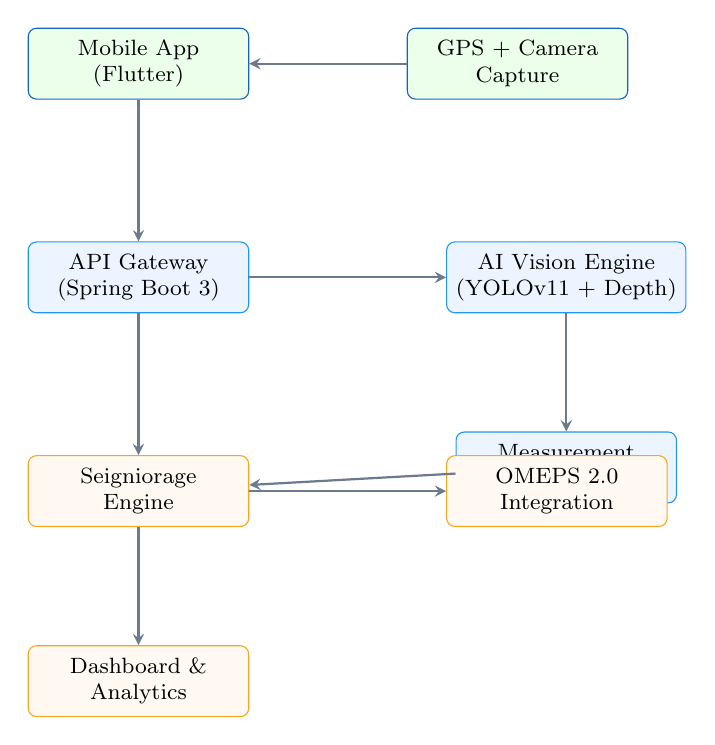
\begin{tikzpicture}[
  node distance=1.2cm and 2cm,
  box/.style={draw, rounded corners=3pt, minimum width=2.8cm, minimum height=0.9cm, align=center, font=\footnotesize},
  field/.style={box, fill=green!8, draw=sectionblue},
  ai/.style={box, fill=pwlight, draw=pwblue},
  gov/.style={box, fill=orange!5, draw=pworange},
  arr/.style={->, >=stealth, thick, color=pwgray}
]

\node[field] (mobile) {Mobile App\\(Flutter)};
\node[field, right=2cm of mobile] (gps) {GPS + Camera\\Capture};

\node[ai, below=1.8cm of mobile] (gateway) {API Gateway\\(Spring Boot 3)};
\node[ai, right=2.5cm of gateway] (vision) {AI Vision Engine\\(YOLOv11 + Depth)};
\node[ai, below=1.5cm of vision] (measure) {Measurement\\Engine};

\node[gov, below=1.8cm of gateway] (seigniorage) {Seigniorage\\Engine};
\node[gov, right=2.5cm of seigniorage] (omeps) {OMEPS 2.0\\Integration};
\node[gov, below=1.5cm of seigniorage] (dashboard) {Dashboard \&\\Analytics};

\draw[arr] (mobile) -- (gateway);
\draw[arr] (gps) -- (mobile);
\draw[arr] (gateway) -- (vision);
\draw[arr] (vision) -- (measure);
\draw[arr] (measure) -- (seigniorage);
\draw[arr] (gateway) -- (seigniorage);
\draw[arr] (seigniorage) -- (omeps);
\draw[arr] (seigniorage) -- (dashboard);

\end{tikzpicture}
\end{center}

% ═══════════════════════════════════════════════════════════════
\newpage
\section{AI Measurement Workflow}

The computer vision pipeline processes field photographs through six stages:

\begin{enumerate}[leftmargin=1.5em, itemsep=4pt]
  \item \textbf{Image Quality Validation:} Checks blur, exposure, resolution before processing. Rejects unusable images with guidance for retake.
  \item \textbf{Granite Block Detection:} YOLOv11 identifies and segments individual granite blocks from background (ground, equipment, other blocks).
  \item \textbf{Depth Estimation:} Depth Anything V2 generates monocular depth map. Combined with reference calibration marker for metric scaling.
  \item \textbf{Dimension Estimation:} Geometric analysis extracts Length, Width, and Height from depth map and perspective geometry. Multiple viewpoints improve accuracy.
  \item \textbf{Volume Calculation:} Computed as L × W × H with confidence interval. Handles irregular shapes via convex hull approximation.
  \item \textbf{Classification \& Fee:} Volume mapped to Above/Below Gangsaw category. Applicable seigniorage slab identified per government schedule. Fee calculated automatically.
\end{enumerate}

% ═══════════════════════════════════════════════════════════════
\section{User Journeys}

\textbf{Quarry Operator:} Captures standardized photos of freshly extracted granite blocks using the DRISHTI mobile app. GPS coordinates, Block ID, and quarry details auto-captured. Receives instant AI-estimated dimensions and indicative seigniorage fee. Submits for officer verification.

\textbf{DMGO Officer:} Reviews AI-computed measurements on dashboard. Compares with visual evidence (photos). For high-confidence predictions ($>$90\%), approves directly. For lower confidence, visits site for verification. Reduces physical inspection frequency by 70\%.

\textbf{Mining Department:} Views district-wise seigniorage analytics. Identifies quarries with anomalous measurement patterns (AI vs.\ weighbridge discrepancy). Triggers audit for revenue recovery. Tracks monthly collection trends and forecasts.

% ═══════════════════════════════════════════════════════════════
\section{Success Metrics}

\begin{itemize}[leftmargin=1.5em, itemsep=4pt]
  \item Granite dimension estimation accuracy $>$\textbf{95\%} (within 5cm of actual measurement).
  \item Volume estimation accuracy $>$\textbf{90\%} (validated against manual measurement baseline).
  \item AI confidence score $>$\textbf{85\%} for 80\%+ of blocks photographed under standard conditions.
  \item Physical inspection reduction of \textbf{70\%} for routine measurements.
  \item Processing time $<$\textbf{30 seconds} from image upload to dimension result.
  \item OMEPS 2.0 integration operational with \textbf{100\%} data synchronization.
  \item Revenue leakage reduction---measurable improvement in seigniorage collection per quarry.
\end{itemize}

% ═══════════════════════════════════════════════════════════════
\newpage
\section{Risks and Mitigations}

\begin{itemize}[leftmargin=1.5em, itemsep=4pt]
  \item \textbf{Variable quarry conditions:} Dust, uneven lighting, and wet surfaces affect image quality. Mitigate with real-time quality validation, LED flash guidance, and model training on diverse field conditions.
  \item \textbf{Irregular block shapes:} Not all blocks are perfect cuboids. Use convex hull volume estimation and flag irregular blocks for manual measurement with lower confidence score.
  \item \textbf{GPS spoofing:} Fake locations could enable fraud. Implement multi-factor validation: GPS + cell tower triangulation + photo metadata cross-check + timestamp sequencing.
  \item \textbf{Network connectivity at quarries:} Remote quarries may lack internet. Offline capture with secure local storage; auto-sync when connectivity returns. Tamper-evident local storage prevents data modification.
  \item \textbf{Calibration accuracy:} Reference marker essential for metric accuracy. Standard government-issued calibration boards placed alongside blocks. Model detects missing/damaged markers.
\end{itemize}

% ═══════════════════════════════════════════════════════════════
\section{Why PeopleWave}

PeopleWave combines computer vision expertise with cloud-native architecture and AP governance domain knowledge. We have delivered AI solutions for RTIH and understand the integration requirements of government systems like OMEPS 2.0.

For Project DRISHTI, our team brings experience in mobile AI deployment, depth estimation models, and GPS-validated field data capture---all critical for a solution that must work reliably at quarry sites across Andhra Pradesh's diverse terrain and conditions.

DRISHTI is designed not as a hackathon demo but as a deployment-ready solution capable of supporting statewide granite measurement and transparent mineral revenue governance.

\vspace{2em}
\begin{flushright}
\textbf{Bhargav Nanekalva}\\
Founder \& CEO, PeopleWave
\end{flushright}

\end{document}
